\documentclass[11pt,compress,t,notes=noshow, xcolor=table]{beamer}
\usepackage[]{graphicx}\usepackage[]{color}
% maxwidth is the original width if it is less than linewidth
% otherwise use linewidth (to make sure the graphics do not exceed the margin)
\makeatletter
\def\maxwidth{ %
  \ifdim\Gin@nat@width>\linewidth
    \linewidth
  \else
    \Gin@nat@width
  \fi
}
\makeatother

\definecolor{fgcolor}{rgb}{0.345, 0.345, 0.345}
\newcommand{\hlnum}[1]{\textcolor[rgb]{0.686,0.059,0.569}{#1}}%
\newcommand{\hlstr}[1]{\textcolor[rgb]{0.192,0.494,0.8}{#1}}%
\newcommand{\hlcom}[1]{\textcolor[rgb]{0.678,0.584,0.686}{\textit{#1}}}%
\newcommand{\hlopt}[1]{\textcolor[rgb]{0,0,0}{#1}}%
\newcommand{\hlstd}[1]{\textcolor[rgb]{0.345,0.345,0.345}{#1}}%
\newcommand{\hlkwa}[1]{\textcolor[rgb]{0.161,0.373,0.58}{\textbf{#1}}}%
\newcommand{\hlkwb}[1]{\textcolor[rgb]{0.69,0.353,0.396}{#1}}%
\newcommand{\hlkwc}[1]{\textcolor[rgb]{0.333,0.667,0.333}{#1}}%
\newcommand{\hlkwd}[1]{\textcolor[rgb]{0.737,0.353,0.396}{\textbf{#1}}}%
\let\hlipl\hlkwb

\usepackage{framed}
\makeatletter
\newenvironment{kframe}{%
 \def\at@end@of@kframe{}%
 \ifinner\ifhmode%
  \def\at@end@of@kframe{\end{minipage}}%
  \begin{minipage}{\columnwidth}%
 \fi\fi%
 \def\FrameCommand##1{\hskip\@totalleftmargin \hskip-\fboxsep
 \colorbox{shadecolor}{##1}\hskip-\fboxsep
     % There is no \\@totalrightmargin, so:
     \hskip-\linewidth \hskip-\@totalleftmargin \hskip\columnwidth}%
 \MakeFramed {\advance\hsize-\width
   \@totalleftmargin\z@ \linewidth\hsize
   \@setminipage}}%
 {\par\unskip\endMakeFramed%
 \at@end@of@kframe}
\makeatother

\definecolor{shadecolor}{rgb}{.97, .97, .97}
\definecolor{messagecolor}{rgb}{0, 0, 0}
\definecolor{warningcolor}{rgb}{1, 0, 1}
\definecolor{errorcolor}{rgb}{1, 0, 0}
\newenvironment{knitrout}{}{} % an empty environment to be redefined in TeX

\usepackage{alltt}
\newcommand{\SweaveOpts}[1]{}  % do not interfere with LaTeX
\newcommand{\SweaveInput}[1]{} % because they are not real TeX commands
\newcommand{\Sexpr}[1]{}       % will only be parsed by R
\newcommand{\xmark}{\ding{55}}%


\usepackage[english]{babel}
\usepackage[utf8]{inputenc}

\usepackage{dsfont}
\usepackage{verbatim}
\usepackage{amsmath}
\usepackage{amsfonts}
\usepackage{amssymb}
\usepackage{bm}
\usepackage{csquotes}
\usepackage{multirow}
\usepackage{longtable}
\usepackage{booktabs}
\usepackage{enumerate}
\usepackage[absolute,overlay]{textpos}
\usepackage{psfrag}
\usepackage{algorithm}
\usepackage{algpseudocode}
\usepackage{eqnarray}
\usepackage{arydshln}
\usepackage{tabularx}
\usepackage{placeins}
\usepackage{tikz}
\usepackage{setspace}
\usepackage{colortbl}
\usepackage{mathtools}
\usepackage{wrapfig}
\usepackage{bm}
\usepackage{amsmath}
\usepackage{pifont}
\usepackage{xcolor} %colored math symbols

\usetikzlibrary{shapes,arrows,automata,positioning,calc,chains,trees, shadows}
\tikzset{
  %Define standard arrow tip
  >=stealth',
  %Define style for boxes
  punkt/.style={
    rectangle,
    rounded corners,
    draw=black, very thick,
    text width=6.5em,
    minimum height=2em,
    text centered},
  % Define arrow style
  pil/.style={
    ->,
    thick,
    shorten <=2pt,
    shorten >=2pt,}
}

\usepackage{subfig}

% Defines macros and environments
\usepackage{../../style/lmu-lecture}


\let\code=\texttt
\let\proglang=\textsf

\setkeys{Gin}{width=0.9\textwidth}

\setbeamertemplate{frametitle}{\expandafter\uppercase\expandafter\insertframetitle}

\usepackage{bbm}
% basic latex stuff
\newcommand{\pkg}[1]{{\fontseries{b}\selectfont #1}} %fontstyle for R packages
\newcommand{\lz}{\vspace{0.5cm}} %vertical space
\newcommand{\dlz}{\vspace{1cm}} %double vertical space
\newcommand{\oneliner}[1] % Oneliner for important statements
{\begin{block}{}\begin{center}\begin{Large}#1\end{Large}\end{center}\end{block}}


%new environments
\newenvironment{vbframe}  %frame with breaks and verbatim
{
 \begin{frame}[containsverbatim,allowframebreaks]
}
{
\end{frame}
}

\newenvironment{vframe}  %frame with verbatim without breaks (to avoid numbering one slided frames)
{
 \begin{frame}[containsverbatim]
}
{
\end{frame}
}

\newenvironment{blocki}[1]   % itemize block
{
 \begin{block}{#1}\begin{itemize}
}
{
\end{itemize}\end{block}
}

\newenvironment{fragileframe}[2]{  %fragile frame with framebreaks
\begin{frame}[allowframebreaks, fragile, environment = fragileframe]
\frametitle{#1}
#2}
{\end{frame}}


\newcommand{\myframe}[2]{  %short for frame with framebreaks
\begin{frame}[allowframebreaks]
\frametitle{#1}
#2
\end{frame}}

\newcommand{\remark}[1]{
  \textbf{Remark:} #1
}


\newenvironment{deleteframe}
{
\begingroup
\usebackgroundtemplate{
\includegraphics[width=\paperwidth,height=\paperheight]{../style/color/red.png}}
 \begin{frame}
}
{
\end{frame}
\endgroup
}
\newenvironment{simplifyframe}
{
\begingroup
\usebackgroundtemplate{
\includegraphics[width=\paperwidth,height=\paperheight]{../style/color/yellow.png}}
 \begin{frame}
}
{
\end{frame}
\endgroup
}\newenvironment{draftframe}
{
\begingroup
\usebackgroundtemplate{
\includegraphics[width=\paperwidth,height=\paperheight]{../style/color/green.jpg}}
 \begin{frame}
}
{
\end{frame}
\endgroup
}
% https://tex.stackexchange.com/a/261480: textcolor that works in mathmode
\makeatletter
\renewcommand*{\@textcolor}[3]{%
  \protect\leavevmode
  \begingroup
    \color#1{#2}#3%
  \endgroup
}
\makeatother


\input{../../latex-math/basic-math}
\input{../../latex-math/basic-ml}
\input{../../latex-math/ml-nn}

\newcommand{\titlefigure}{figure/difficult_vs_easy_intro.png}
\newcommand{\learninggoals}{
  \item Ill-Conditioning
  \item Local Minima
  \item Saddle Points
  \item Cliffs and Exploding Gradients
}

\title{Deep Learning}
\date{}

\begin{document}

\lecturechapter{Challenges in Optimization}
\lecture{I2DL}

\begin{frame}{Challenges in Optimization}
 \begin{itemize}
   \item In this section, we summarize several of the most prominent challenges regarding training of deep neural networks.
   \item Traditionally, machine learning ensures that the optimization problem is convex by carefully designing
the objective function and constraints. But for neural networks we are confronted with the general nonconvex case. 
   \item Furthermore, we will see in this section that even convex optimization is not without its complications.
 \end{itemize}
\end{frame}

%%%%%%%%%%%%%%%%%%%%%%%%%%%%%%%%%%%%%%%%%%%%%%%%%%%%%%%%%%%%%%%%%%
\section{Ill-Conditioning}

\begin{frame} {Effects of curvature}

Intuitively, the curvature of a function determines the outcome of a GD step\dots


\vspace*{-0.5cm}
\begin{figure}
\captionsetup{font=footnotesize,labelfont=footnotesize, labelfont = bf}
\begin{center}
	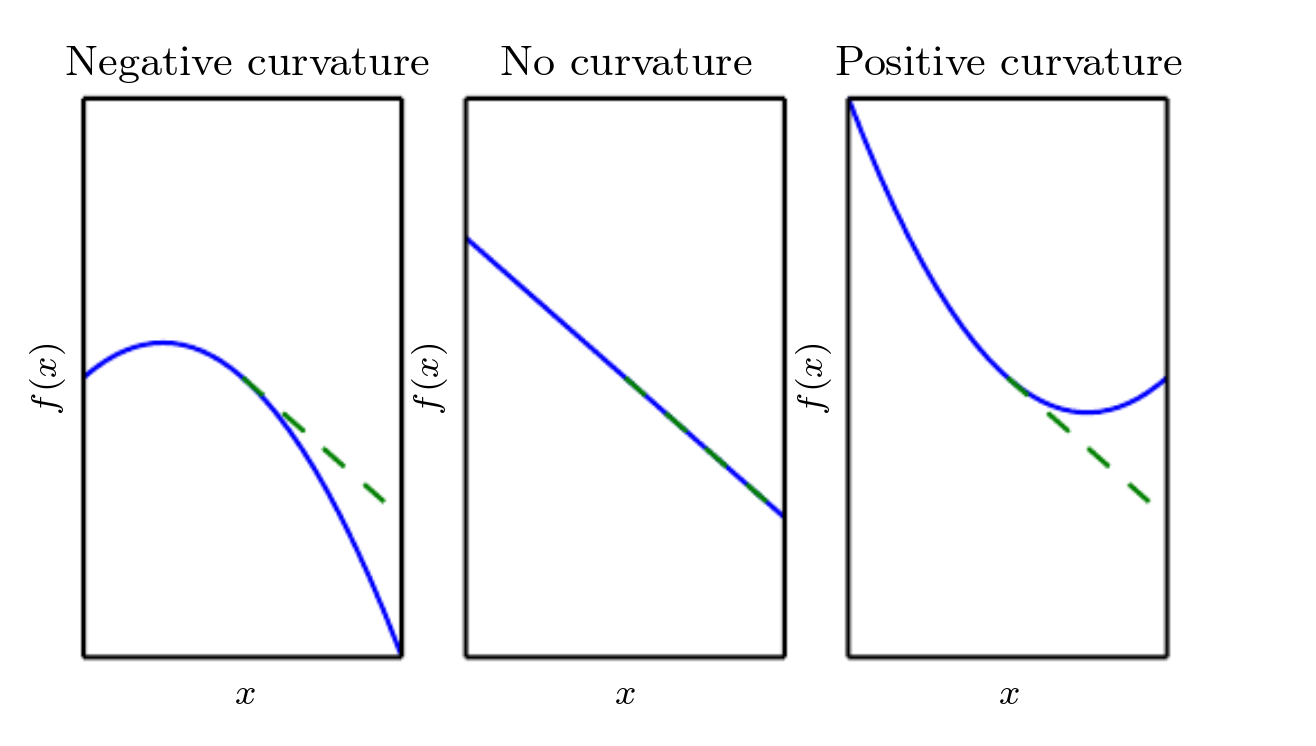
\includegraphics[width=.7\textwidth]{figure/curvature.png}
\end{center}
\tiny{Source: Goodfellow \emph{et al.}, (2016), ch. 4}
\caption{Quadratic objective function $\fx$ with various curvatures.
The dashed line indicates the first order taylor approximation based on the gradient information alone. Left: With negative curvature, the cost function decreases faster than the gradient predicts; Middle: With no curvature, the gradient predicts the decrease correctly; Right: With positive curvature, the function decreases more slowly than expected and begins to increase. }
\end{figure}
\end{frame}

\begin{vbframe}{Second derivative and curvature}

To understand better how the curvature of a function influences the outcome of a gradient descent step, let us recall how curvature is described mathematically: 

\begin{itemize}
  \item The second derivative corresponds to the curvature of the graph of a function. 
  \item The \textbf{Hessian} matrix of a function $\riskt: \mathbb{R}^m \to \mathbb{R}$ is the matrix of second-order partial derivatives
  $$
    H_{ij} = \frac{\partial^2}{\partial \theta_i \partial \theta_j} \riskt.
  $$
\end{itemize}

\framebreak 

\begin{itemize}
  \item The second derivative in a direction $\mathbf{d}$, %of length $1$
   with $\|\mathbf{d}\| = 1$, is given by $\mathbf{d}^\top \!\Hess\,\mathbf{d}$.
  \item What is the direction of the highest curvature (red direction), and what is the direction of the lowest curvature (blue)?
\end{itemize}

\vspace*{-0.5cm}

\begin{figure}
\begin{center}
  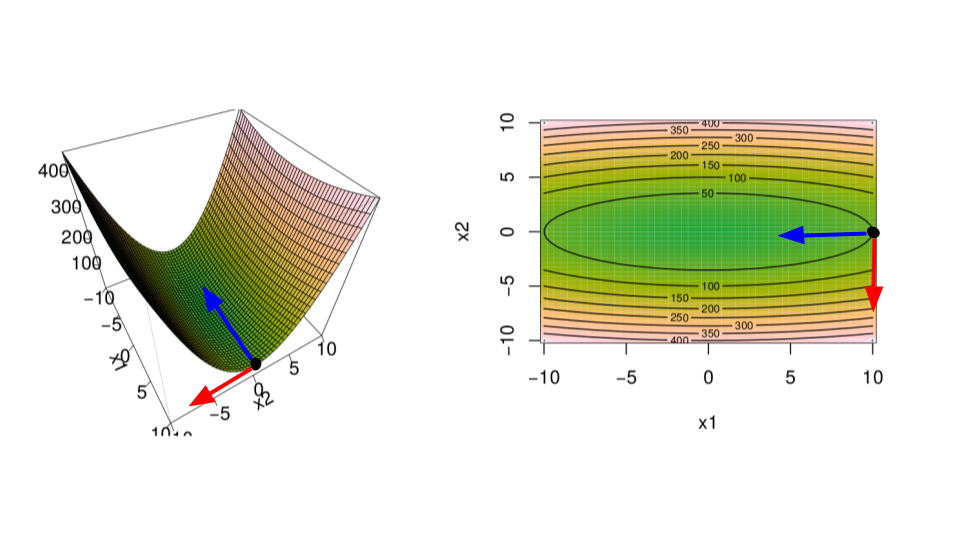
\includegraphics{figure/curvature2.png}
\end{center}
\end{figure}

\framebreak

\begin{itemize}
  \item Since $\Hess$ is real and symmetric (why?), eigendecomposition yields
  $\Hess = \mathbf{V} \mathbf{\diag(\boldsymbol{\lambda})} \mathbf{V}^{-1}$
  with $\mathbf{V}$ and $\boldsymbol{\lambda}$ collecting eigenvectors and eigenvalues, respectively.
  \item It can be shown, that the eigenvector $\textcolor{red}{\bm{v}_{\text{max}}}$ with the max. eigenvalue $\lambda_{\text{max}}$ points into the direction of highest curvature ($\bm{v}_{\text{max}}^\top \bm{H} \bm{v}_{\text{max}} = \lambda_{\text{max}}$), while the eigenvector $\textcolor{blue}{\bm{v}_{\text{min}}}$ with the min. eigenvalue $\lambda_{\text{min}}$ points into the direction of least curvature. 
\end{itemize}

\vspace*{-0.5cm}

\begin{figure}
  \begin{center}
    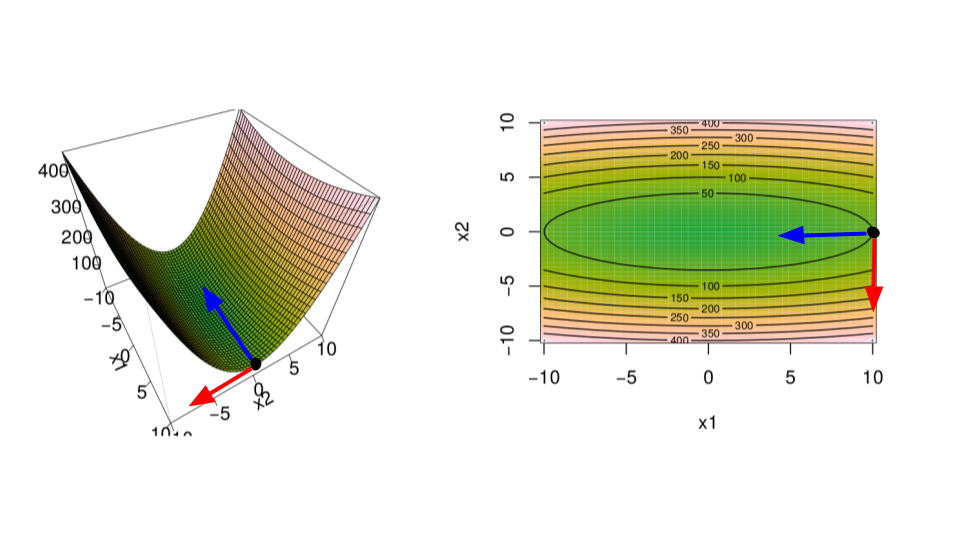
\includegraphics[width=.7\textwidth]{figure/curvature2.png}
  \end{center}
\end{figure}

\framebreak 

\begin{itemize}
  \item At a stationary point $\thetav$, where the gradient is 0, we can examine the eigenvalues of the Hessian to determine whether the $\thetav$ is a local maximum, minimum or saddle point: 
  \vspace{-0.3cm}
  \begin{align*} 
  \quad\forall i: \lambda_i > 0  \, (\Hess \text{ positive definite at $\thetav$}) &\quad\Rightarrow\quad \text{minimum at $\thetav$} \\
  \quad\forall i: \lambda_i < 0 \, (\Hess \text{ negative definite at $\thetav$}) &\quad\Rightarrow\quad \text{maximum at $\thetav$}\\
  \exists\, i: \lambda_i < 0 \land  \exists j: \lambda_j > 0  \,(\Hess \text{ indefinit at $\thetav$}) &\quad\Rightarrow\quad \mbox{saddle point at $\thetav$}
  \end{align*}
\end{itemize}
   \begin{figure}
 \captionsetup{font=footnotesize,labelfont=footnotesize, labelfont = bf}

 \begin{center}
  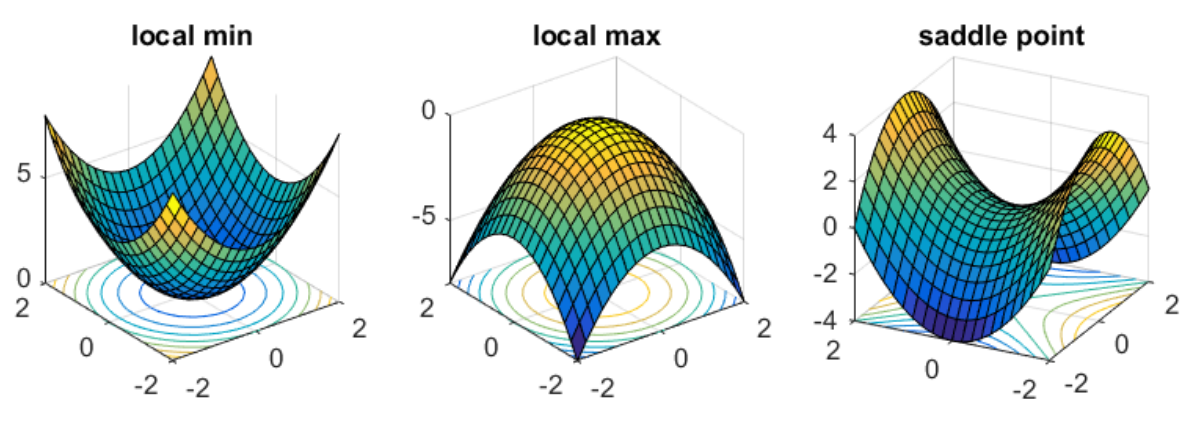
\includegraphics[width=.7\textwidth]{figure/3dim_curvature.png}
 \end{center}
 \tiny{Credit: Rong Ge (2016)}
 \end{figure}

 \end{vbframe}

 \begin{vbframe}{Ill-conditioned Hessian matrix} 


 The condition number of a symmetric matrix $\bm{A}$ is given by the ratio of its min/max eigenvalues $\kappa(\bm{A}) = \frac{|\lambda_{\text{max}}|}{|\lambda_{\text{min}}|}$. A matrix is called ill-conditioned, if the condition number $\kappa(\bm{A})$ is very high. 

 \lz 

 An \textbf{ill-conditioned} Hessian matrix means that the ratio of max. / min. curvature is high, as in the example below: 

\begin{center}
  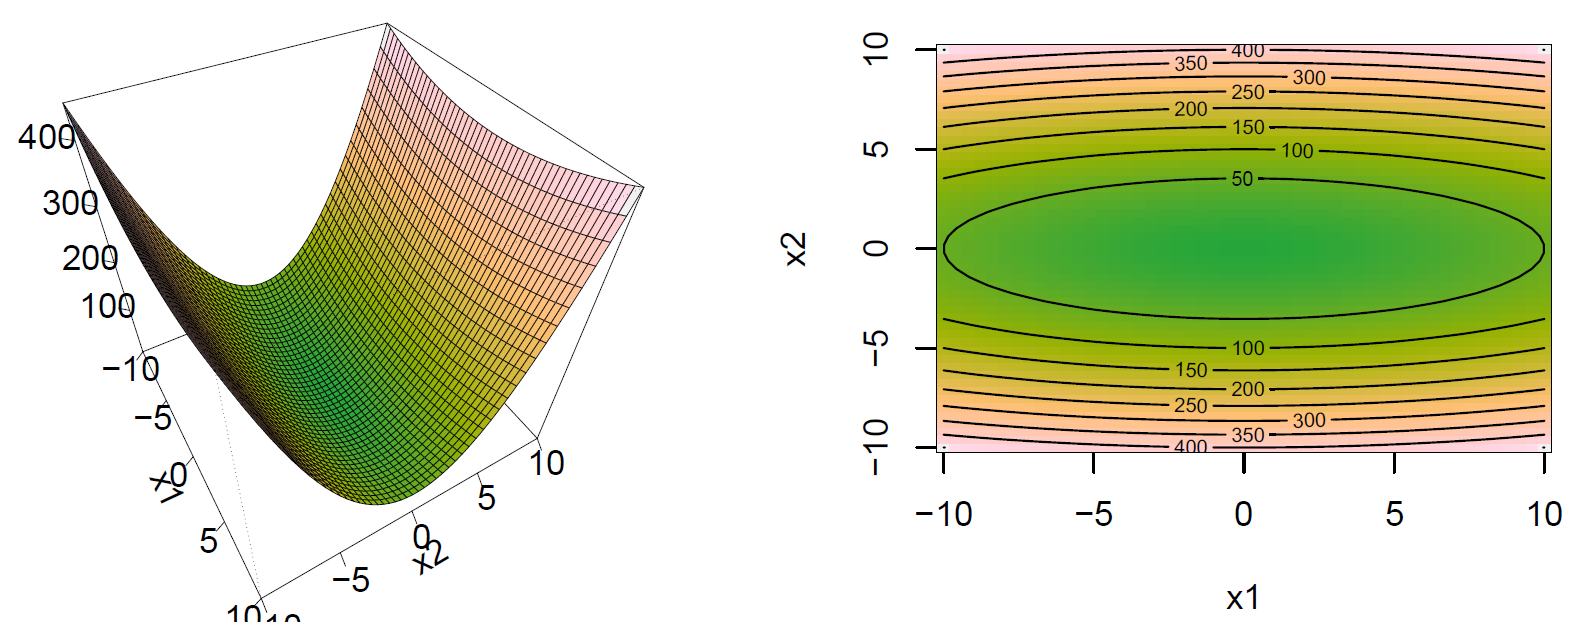
\includegraphics[width=0.7\textwidth]{figure/ill-con.png}
\end{center}


\end{vbframe}

\begin{vbframe}{Curvature and Step-size in GD}

What does it mean for gradient descent if the Hessian is ill-conditioned?

 \begin{itemize}
 \item Let us consider the second-order Taylor approximation as a local approximation of the of $\risk$ around a current point $\boldsymbol{\theta}^0$ (with gradient $\mathbf{g}$)
    \begin{equation*}
    \risk(\boldsymbol{\theta}) \approx T_2f(\thetav, \boldsymbol{\theta}^0) := \risk(\boldsymbol{\theta}^0) + (\boldsymbol{\theta}-\boldsymbol{\theta}^0)^\top \mathbf{g} + \frac{1}{2}(\boldsymbol{\theta}-\boldsymbol{\theta}^0)^\top \!\Hess\, (\boldsymbol{\theta}-\boldsymbol{\theta}^0)
    \end{equation*}
  \item Furthermore, Taylor's theorem states (proof in Koenigsberger (1997), p. 68)
    \begin{equation*}
     \underset{\thetav \rightarrow \boldsymbol{\theta}^0}{\lim} \frac{\risk(\thetav) - T_2f(\thetav, \boldsymbol{\theta}^0)}{||\thetav-\boldsymbol{\theta}^0||^2} = 0
   \end{equation*}

  \framebreak 

  \item One GD step with a learning rate $\alpha$ yields new parameters $\boldsymbol{\theta}^0-\alpha \mathbf{g}$ and a new approximated loss value
   $$
   \risk(\boldsymbol{\theta}^0-\alpha \mathbf{g}) \approx \risk(\boldsymbol{\theta}^0) - \alpha \mathbf{g}^\top\mathbf{g} + \frac{1}{2}	\alpha^2 \mathbf{g}^\top\!\Hess\,\mathbf{g}  \,.
   $$ 
 
 \item Theoretically, if $\mathbf{g}^\top \Hess \mathbf{g}$ is positive, we can solve the equation above for the optimal step size which corresponds to 
 $$
 \alpha^* = \frac{\mathbf{g}^\top \mathbf{g}}{\mathbf{g}^\top \!\Hess\, \mathbf{g}}  \,.
 $$
 
 \framebreak 

 \item Let us assume the gradient $\mathbf{g}$ points into the direction of $\bm{v}_{\text{max}}$ (i.e. the direction of highest curvature), the optimal step size is given by 
  $$
  \alpha^* = \frac{\mathbf{g}^\top \mathbf{g}}{\mathbf{g}^\top \!\Hess\, \mathbf{g}} = \frac{\mathbf{g}^\top \mathbf{g}}{\lambda_{\text{max}} \mathbf{g}^\top   \mathbf{g}} = \frac{1}{\lambda_{\text{max}}}, 
  $$ 
  which is very small. Choosing a too large step-size is bad, as it will make us \enquote{overshoot} the stationary point.
  \item If, on the other hand, $\mathbf{g}$ points into the direction of the lowest curvature, the optimal step size is 
  $$
  \alpha^* = \frac{1}{\lambda_{\text{min}}}, 
  $$
  which corresponds to the largest possible optimal step-size.
  \item We summarize: We want to perform big steps in directions of low curvature, but small steps in directions of high curvature.

  \framebreak 

  \item But what if the gradient does not point into the direction of one of the eigenvectors? 
  \item Let us consider the 2-dimensional case: We can decompose the direction of $\bm{g}$ (black) into the two eigenvectors $\textcolor{red}{\bm{v}_{\text{max}}}$ and $\textcolor{blue}{\bm{v}_{\text{min}}}$
  \item It would be optimal to perform a \textbf{big} step into the direction of the smallest curvature $\textcolor{blue}{\bm{v}_{\text{min}}}$, but a \textbf{small} step into the direction of $\textcolor{red}{\bm{v}_{\text{max}}}$, but the gradient points into a completely different direction. 
  \end{itemize}

  \vspace*{-0.4cm}

  \begin{figure}
    \begin{center}
      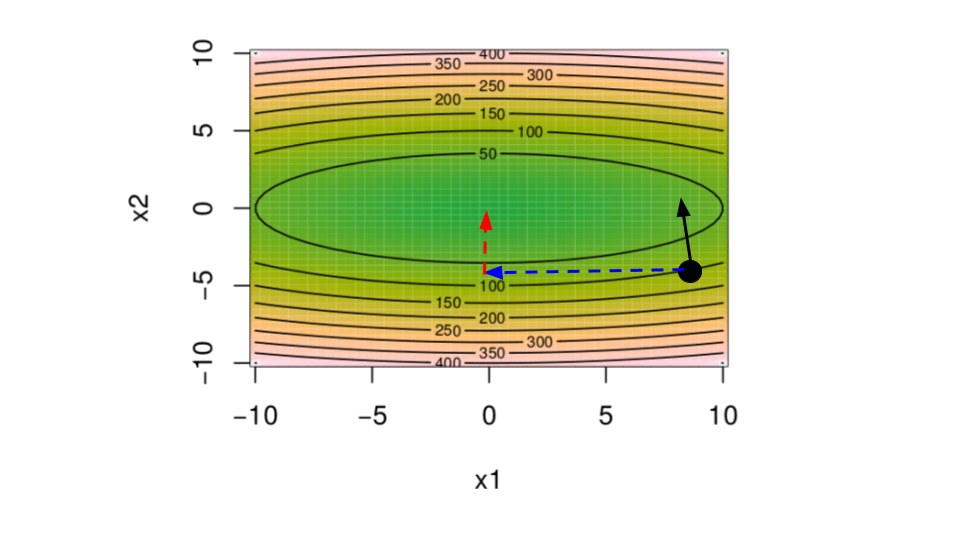
\includegraphics[width=.7\textwidth]{figure/curvature3.png}
    \end{center}
  \end{figure}

\end{vbframe}

% \begin{frame} {Effects of curvature}
% \begin{itemize}
% \item The second-order Taylor approximation (with gradient $\mathbf{g}$) around current point $\boldsymbol{\theta}^0$ is
% \begin{equation*}
% \risk(\boldsymbol{\theta}) = \risk(\boldsymbol{\theta}^0) + (\boldsymbol{\theta}-\boldsymbol{\theta}^0)^\top \mathbf{g} + \frac{1}{2}(\boldsymbol{\theta}-\boldsymbol{\theta}^0)^\top \!\Hess\, (\boldsymbol{\theta}-\boldsymbol{\theta}^0)
% \end{equation*}
% \item SGD with learning rate $\alpha$ yields new parameters $\boldsymbol{\theta}^0-\alpha g$ and new loss value
% $$
% \risk(\boldsymbol{\theta}^0-\alpha \mathbf{g}) = \risk(\boldsymbol{\theta}^0) - \alpha \mathbf{g}^\top\mathbf{g} + \frac{1}{2}	\alpha^2 \mathbf{g}^\top\!\Hess\,\mathbf{g}  \,.
% $$
% \item When $g^\top H g$ is to large, we might get $\risk(\boldsymbol{\theta}^0-\alpha \mathbf{g}) > \risk(\boldsymbol{\theta}^0)$.
% \item If $\mathbf{g}^\top \Hess \mathbf{g}$ is positive, optimal step size is
% $$
% \alpha^* = \frac{\mathbf{g}^\top \mathbf{g}}{\mathbf{g}^\top \!\Hess\, \mathbf{g}} \ge \frac{1}{\lambda_{\text{max}}}  \,.
% $$
% \end{itemize}
% \end{frame}

\begin{vbframe} {Ill-conditioning}


\begin{itemize}
  %   \item The new risk after a \textbf{gradient descent} step is 
  %   $$
  %   \risk(\boldsymbol{\theta}^0-\alpha \mathbf{g}) \approx \risk(\boldsymbol{\theta}^0) \underbrace{- \alpha \mathbf{g}^\top\mathbf{g} + \frac{1}{2}	\alpha^2 \mathbf{g}^\top\!\Hess\,\mathbf{g}}_{:=\nu}  \,.
  %   $$ 
  % The term  $\nu$ is added to the risk $\risk$ in each gradient descent step. 
  %   \item Ill-conditioning of the Hessian matrix $\Hess$ becomes a problem, when $$\frac{1}{2}	\alpha^2 \mathbf{g}^\top\!\Hess\,\mathbf{g}^\top > \alpha \mathbf{g}^\top\mathbf{g}$$
  %   \item Ill-conditioning occurrs, if the second derivatives for a specific point differ a lot. This can be measured by the condition number. A condition number of 5, for example, means that the direction of the highest curvature has five times more curvature than the direction of the least  curvature. 

  % \framebreak 
  \item GD is unaware of large differences in curvature, and can only walk into the direction of the gradient.  
  \item Choosing a too large step-size will then cause the descent direction change frequently (\enquote{jumping around}).
  \item $\alpha$ needs to be small enough, which results in a low progress.
  
  \framebreak
  
  \item This effect is more severe, if a Hessian has a poor condition number, i.e. the ratio between lowest and highest curvature is large; gradient descent will perform poorly. 
  \begin{figure}
  \captionsetup{font=footnotesize,labelfont=footnotesize, labelfont = bf}
  \begin{center}
  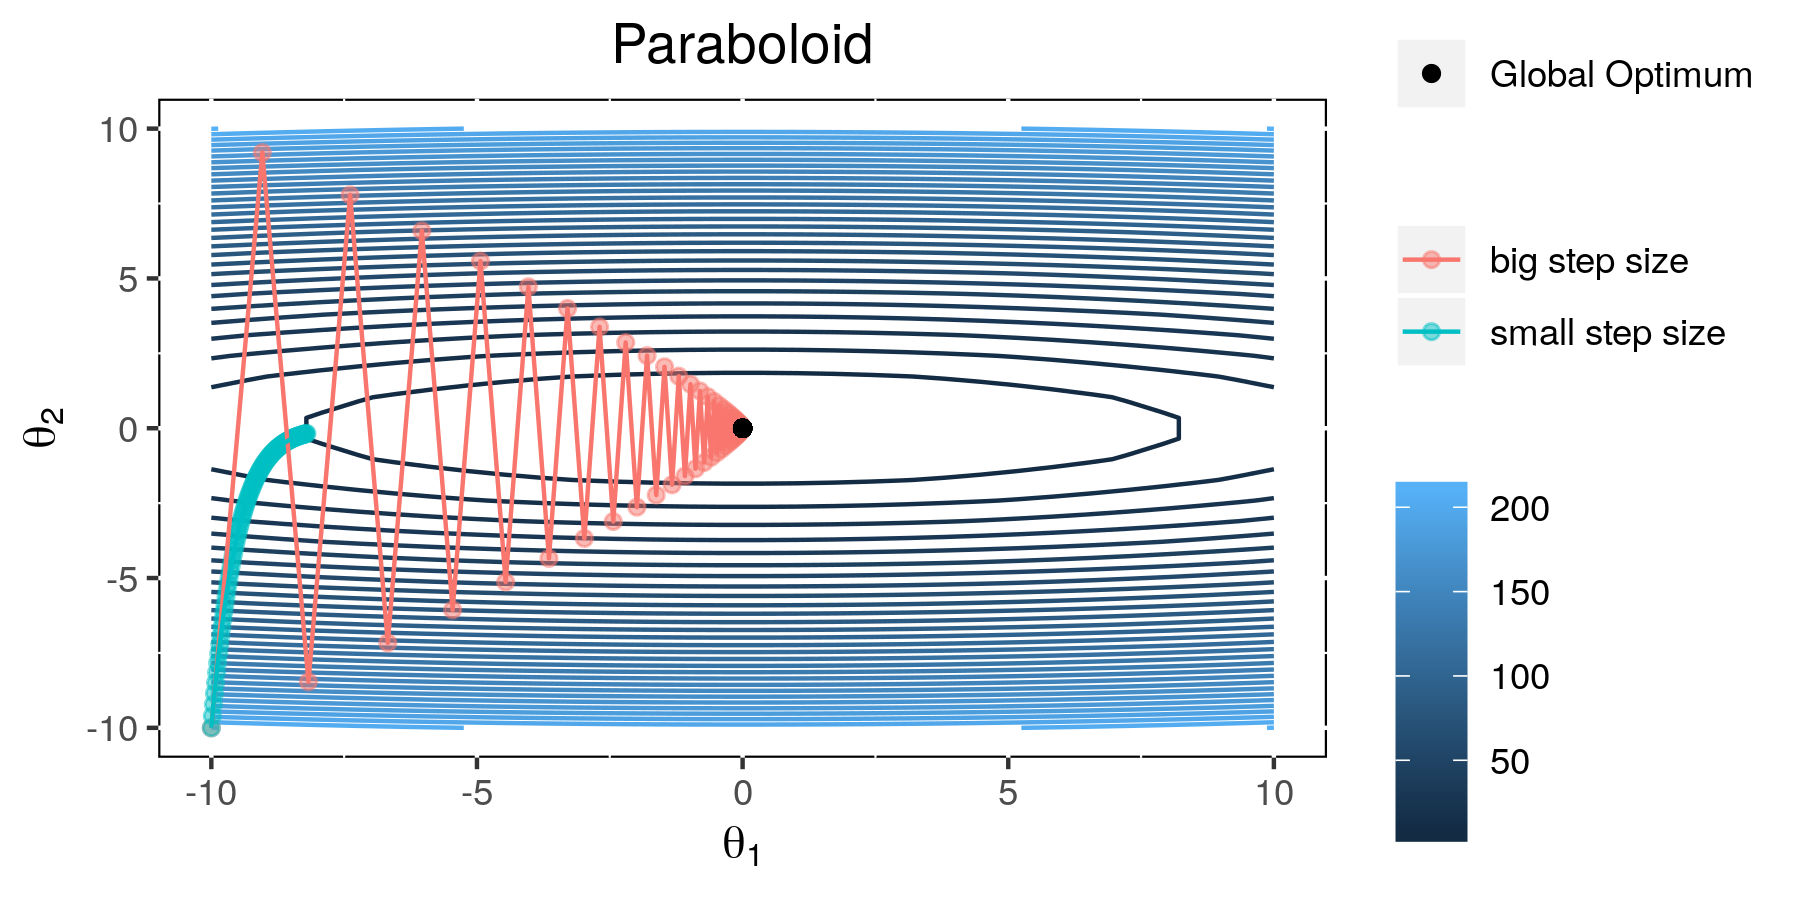
\includegraphics[width=0.7\textwidth]{figure/big_small_stepsize.png}
  \end{center}
  \caption{The contour lines show a quadratic risk function with a poorly conditioned Hessian matrix. The plot shows the progress of gradient descent with a small step-size vs. larger step-size. In both cases, convergence to the global optimum is rather slow. }
  \end{figure}

  \item In the worst case, ill-conditioning of the Hessian matrix and a too big step-size will cause the risk to increase

    $$
   \risk(\boldsymbol{\theta}^0-\alpha \mathbf{g}) \approx \risk(\boldsymbol{\theta}^0) - \alpha \mathbf{g}^\top\mathbf{g} + \frac{1}{2} \alpha^2 \mathbf{g}^\top\!\Hess\,\mathbf{g}  \,,
   $$ 
   which happens if 
   $$
    \frac{1}{2} \alpha^2 \mathbf{g}^\top\!\Hess\,\mathbf{g} > \alpha \mathbf{g}^\top\mathbf{g}.
   $$
    \item To determine whether ill-conditioning is detrimental to the training, the squared gradient norm $\mathbf{g}^\top \mathbf{g}$ and the risk %and the term $\mathbf{g}^\top\Hess\mathbf{g}$ 
    can be monitored.

    \begin{figure}
      \captionsetup{font=footnotesize,labelfont=footnotesize, labelfont = bf}
    \centering
      \scalebox{0.8}{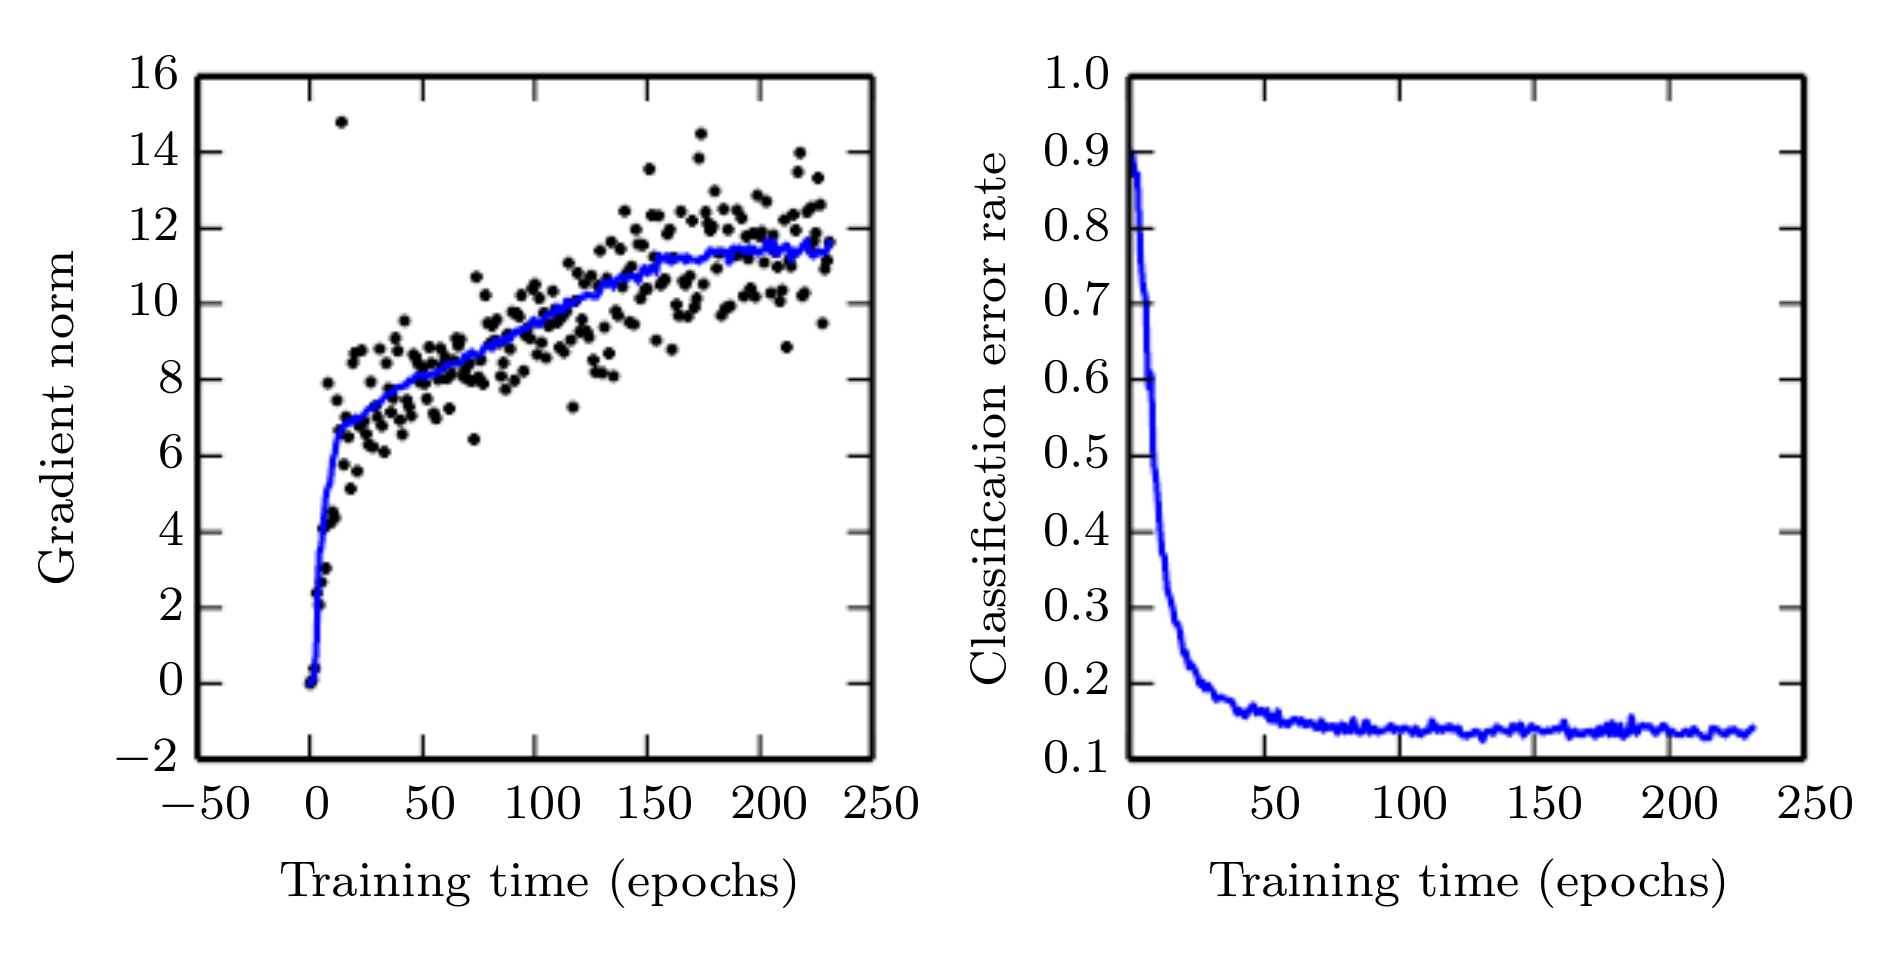
\includegraphics{figure/no_critical.png}}
      \tiny{\\Source: Goodfellow, ch. 6}
    \end{figure}

    \vspace*{-0.1cm}

    \item Gradient norms \textbf{increase} over time, showing that the training process is not converging to a stationary point $\mathbf{g} = 0$. 
    \item At the same time, we observe that the risk is approx. constant, but the gradient norm increases
    \vspace*{-0.2cm}
    $$
      \underbrace{\risk(\boldsymbol{\theta}^0-\alpha \mathbf{g})}_{\text{approx. constant}} \approx \risk(\boldsymbol{\theta}^0) - \underbrace{\alpha \mathbf{g}^\top\mathbf{g}}_{\text{increase}}+ \frac{1}{2}  \underbrace{\alpha^2 \mathbf{g}^\top\!\Hess\,\mathbf{g}}_{\to \text{increase}}  \,. 
     $$ 
  \end{itemize}
\end{vbframe}

%%%%%%%%%%%%%%%%%%%%%%%%%%%%%%%%%%%%%%%%%%%%%%%%%%%%%%%%%%%%%%%
\section{Local Minima}

\begin{vbframe}{Unimodal vs. Multimodal loss surfaces}
  \begin{figure}
  \centering
    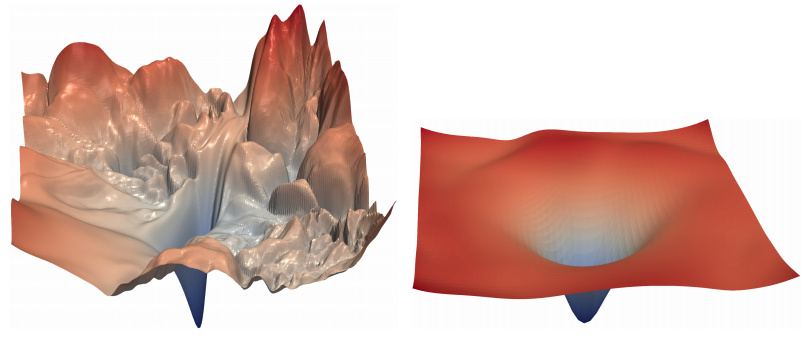
\includegraphics[width=12cm]{figure/difficult_vs_easy.png}
    \caption{Left: Multimodal loss surface with saddle points; Right: (Nearly) unimodal loss surface (Hao Li et al. (2017))}
  \end{figure}
\end{vbframe}

%%%%%%%%%%%%%%%%%%%%%%%%%%%%%%%%%%%%%%%%%%%%%%%%%%%%%%%%%%%%%%%%%%

\begin{vbframe}{Multimodal function}
Potential snippet from a loss surface of a deep neural network with many local minima:

\begin{center}
  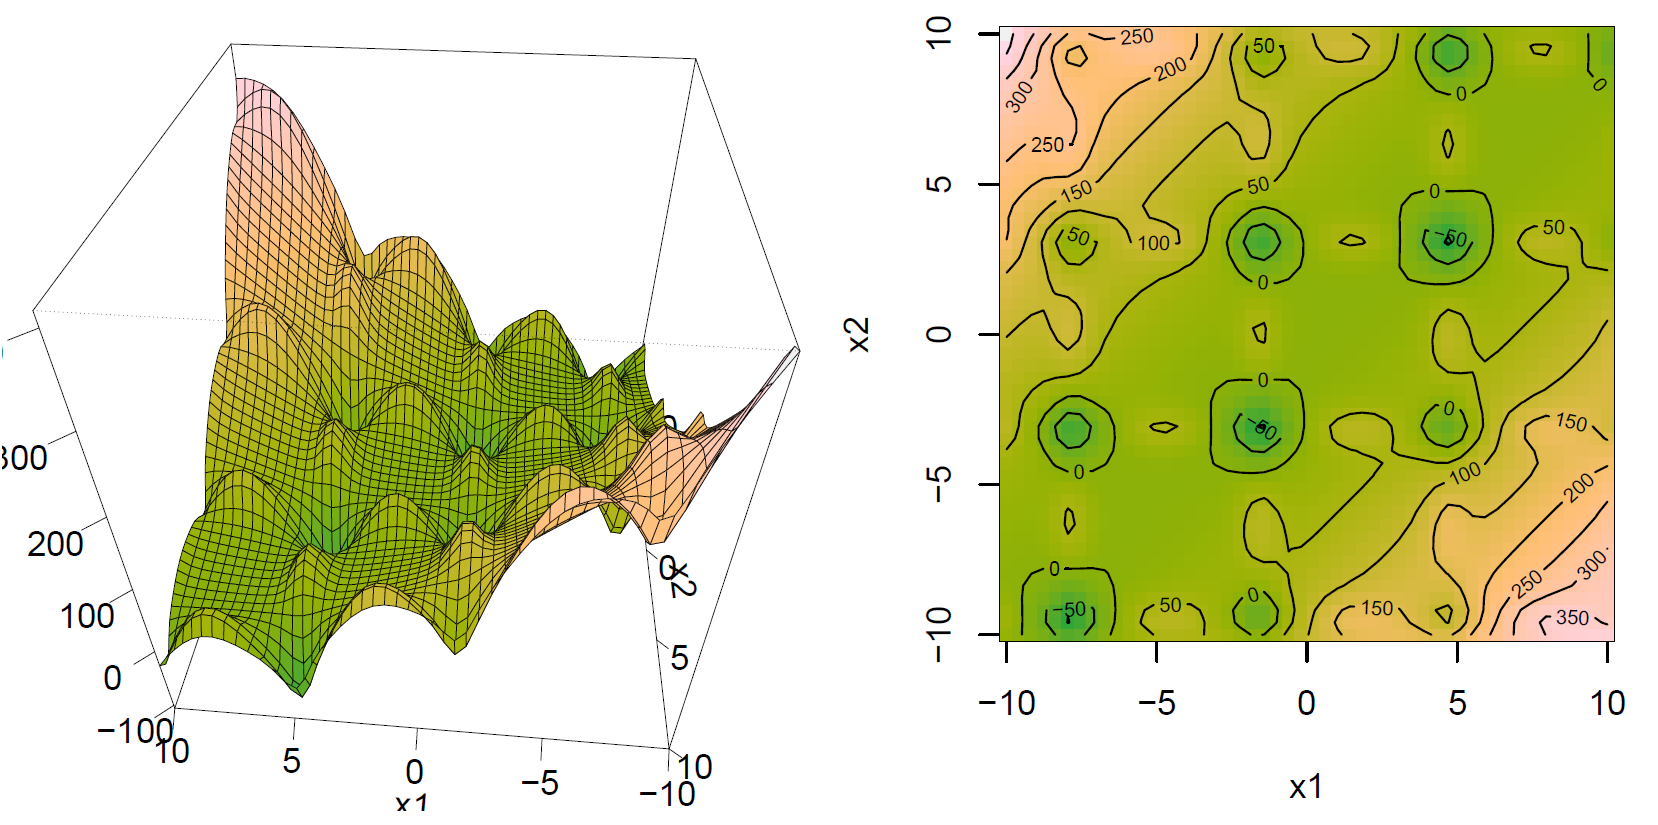
\includegraphics[width=.9\textwidth]{figure/multimodal.png}
\end{center}

\end{vbframe}

\begin{frame} {Only locally optimal moves}
  \begin{itemize}
  \small{
    \item If the training algorithm makes only \textit{locally} optimal moves (as in gradient descent), it may move away from regions of \textit{much} lower cost.
      \begin{figure}
    \centering
      \scalebox{0.65}{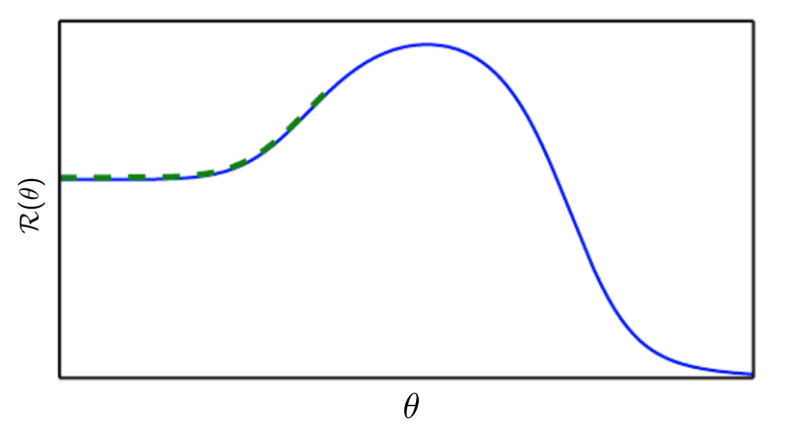
\includegraphics{figure/local_hill.png}}
      \tiny{\\Source: Goodfellow, Ch. 8}
    \end{figure}
    \item In the figure above, initializing the parameter on the "wrong" side of the hill will result in suboptimal performance.
    \item In higher dimensions, however, it may be possible for gradient descent to go around the hill but such a trajectory might be very long and result in excessive training time.}
  \end{itemize}
\end{frame}

\begin{vbframe} {Local minima}
   Weight space symmetry:
   \begin{itemize}
       \item If we swap incoming weight vectors for neuron $i$ and $j$
       and do the same for the outcoming weights,
       modelled function stays unchanged.
        \begin{itemize}
           \item[$\Rightarrow$] with $n$ hidden units and one hidden layer
           there are $n!$ networks with the same empirical risk
        \end{itemize}
       \item If we multiply incoming weights of a ReLU neuron with $\beta$
       and outcoming with $1/\beta$ the modelled function stays unchanged.
      \end{itemize}
  $\Rightarrow$ The empirical risk of a NN can have very many
          minima with equivalent empirical risk.

\framebreak 

    \begin{itemize}
     \item In practice only local minima with a high value compared to the global minimium are problematic.
    \begin{figure}
     \begin{center}
     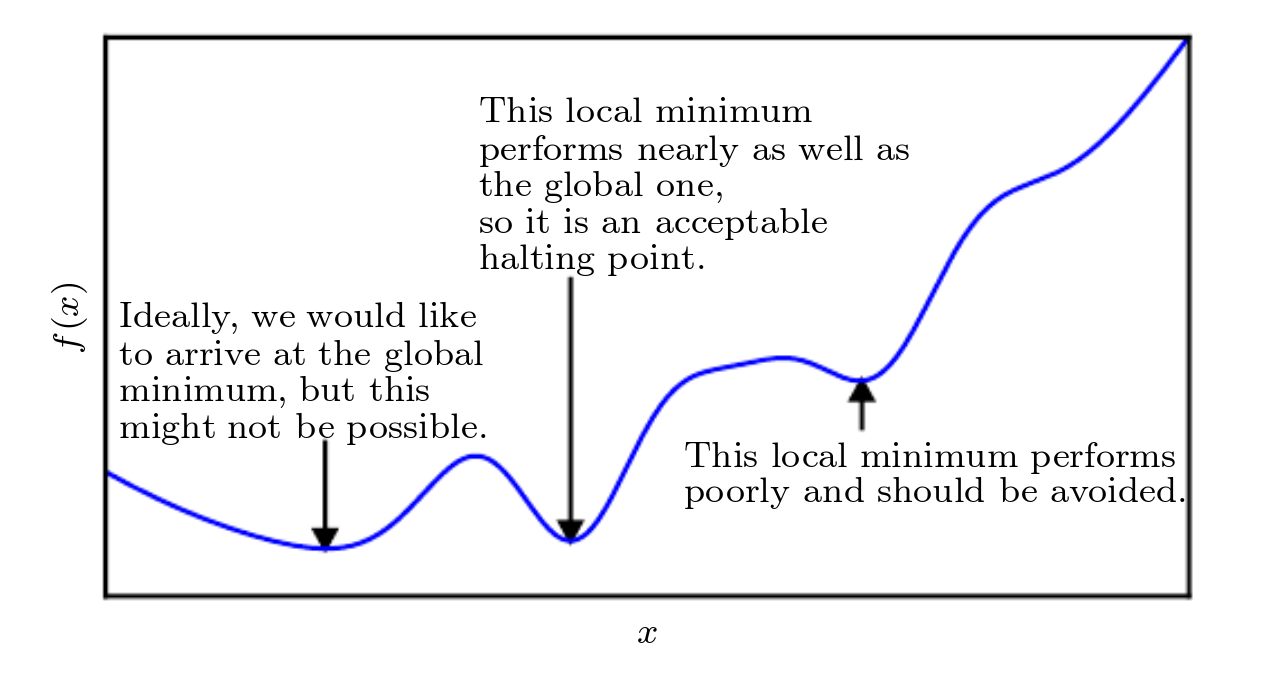
\includegraphics[width=.6\textwidth]{figure/minima.png}
     \end{center}
    \tiny{Source: Goodfellow, Ch. 4}
    \end{figure}
     \item Current literature suspects that most local minima have low empirical risk.
\end{itemize}
\end{vbframe}

%%%%%%%%%%%%%%%%%%%%%%%%%%%%%%%%%%%%%%%%%%%%%%%%%%%%%%%%%%%%%%%%%%
\section{Saddle Points}
\begin{vbframe}{Saddle Points}
  \begin{itemize}
    \item In optimization we look for areas with zero gradient.
    \item A variant of zero gradient areas are saddle points.
    \item For the empirical risk $\risk$ of a neural network, the expected ratio of the number of saddle points to local minima typically grows exponentially with $m$ 
    $$\risk: \mathbb{R}^m \rightarrow \mathbb{R}$$ 
    In other words: Networks with more parameters (deeper networks or larger layers) exhibit a lot more saddle points than local minima.
     \item Why is that?
    \item The Hessian at a local minimum has only positive eigenvalues. At a saddle point it is a mixture of positive and negative eigenvalues.
    
\framebreak
    
    \item Imagine the sign of each eigenvalue is generated by coin flipping:
    \begin{itemize}
      \item In a single dimension, it is easy to obtain a local minimum (e.g. \enquote{head} means positive eigenvalue).
      \item In an $m$-dimensional space, it is exponentially unlikely that all $m$ coin tosses will be head.
    \end{itemize}
    \item A property of many random functions is that eigenvalues of the Hessian become more likely to be positive in regions of lower cost.
    \item For the coin flipping example, this means we are more likely to have heads $m$ times if we are at a critical point with low cost.
    \item That means in particular that local minima are much more likely to have low cost than high cost and critical points with high cost are far more likely to be saddle points.
    \item See Dauphin et al. (2014) for a more detailed investigation.
  \end{itemize}
\end{vbframe}

\begin{vbframe}{Saddle Points: Example}
  \begin{center}
    $f(x_1, x_2) = x_1^2 - x_2^2$
  \end{center}
  \begin{figure}
    \centering
    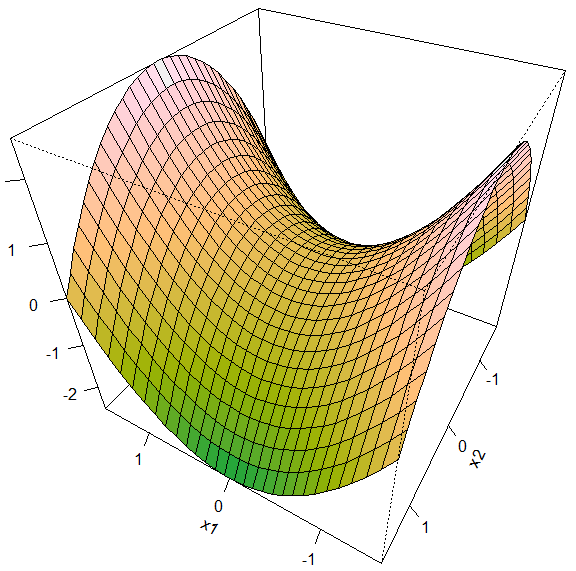
\includegraphics[width=4cm]{figure/saddlepoint.png}
  \end{figure} 
  \begin{itemize}
    \item Along $x_1$, the function curves upwards (eigenvector of the Hessian with positive eigenvalue). Along $x_2$, the function curves downwards (eigenvector of the Hessian with negative eigenvalue).
  \end{itemize}
\end{vbframe}

\begin{vbframe}{Saddle Points}
  \begin{itemize}
    \item So how do saddle points impair optimization?
    \item First-order algorithms that use only gradient information \textbf{might} get stuck in saddle points.
    \item Second-order algorithms experience even greater problems when dealing with saddle points. Newtons method for example actively searches for a region with zero gradient. That might be another reason why second-order methods have not succeeded in replacing gradient descent for neural network training. 
  \end{itemize}
\end{vbframe}

%%%%%%%%%%%%%%%%%%%%%%%%%%%%%%%%%%%%%%%%%%%%%%%%%%%%%%%%%%%

\frame{

\frametitle{Example: Saddle point with GD}

  \center
  \only<1>{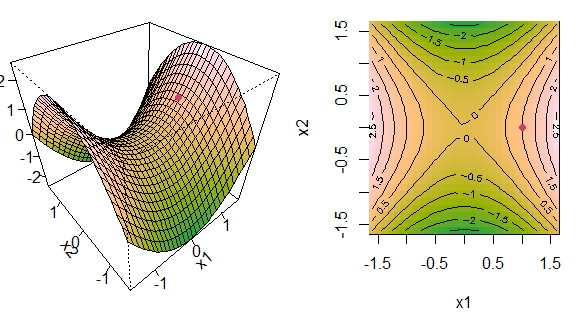
\includegraphics[width=9cm]{figure/opt1.png}}%
  \only<2>{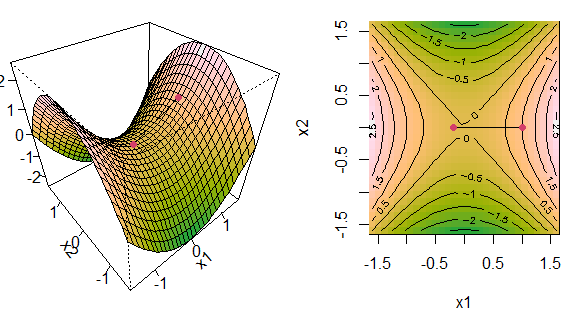
\includegraphics[width=9cm]{figure/opt2.png}}%
  \only<3>{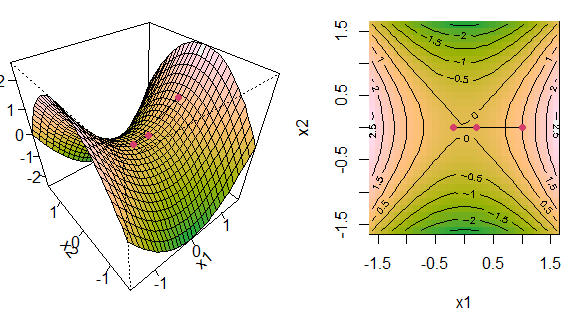
\includegraphics[width=9cm]{figure/opt3.png}}%
  \only<4>{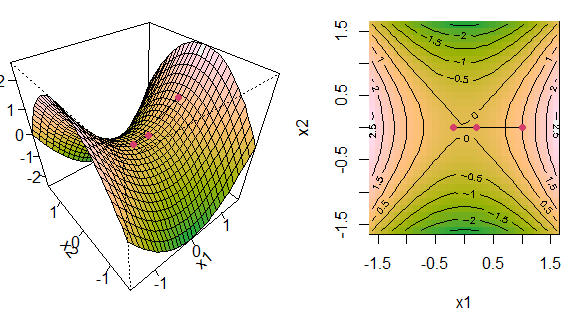
\includegraphics[width=9cm]{figure/opt10.png}}%
  
  \begin{itemize}

    \only<1>{\item[] \small{Red dot: Starting location}}
    \only<2>{\item[] \small{First step...}}
    \only<3>{\item[] \small{...second step...}}
    \only<4>{\item[] \small{...tenth step got stuck and cannot escape the saddle point!}}
    
  \end{itemize}

}

\section{Cliffs and Exploding Gradients}
\begin{vbframe}{Cliffs and exploding gradients}
  \begin{itemize}
    \item As a result from the multiplication of several parameters, the emprirical risk for highly nonlinear deep neural networks often contain sharp nonlinearities.
      \begin{itemize}
        \item That may result in very high derivatives in some places.
        \item As the parameters get close to such cliff regions, a gradient descent update can catapult the parameters very far.
        \item Such an occurrence can lead to losing most of the optimization work that had been done.
      \end{itemize}
    \item However, serious consequences can be easily avoided using a technique called \textbf{gradient
clipping}.
    \item The gradient does not specify the optimal step size, but only the optimal direction
within an infinitesimal region.
\framebreak 
    \item Gradient clipping simply caps the step size to be small enough that it is less likely to go outside the region where the gradient indicates the direction of steepest descent.
    \item We simply \enquote{prune} the norm of the gradient at some threshold $h$:
    $$\text{if  } ||\nabla \thetav|| > \text h: \nabla \thetav \leftarrow \frac{h}{||\nabla \thetav||} \nabla \thetav $$
  \end{itemize}
\end{vbframe}

%%%%%%%%%%%%%%%%%%%%%%%%%%%%%%%%%%%%%%%%%%%%%%%%%%%%%%

\begin{vbframe}{Example: cliffs and exploding gradients}
  \begin{figure}
  \centering
    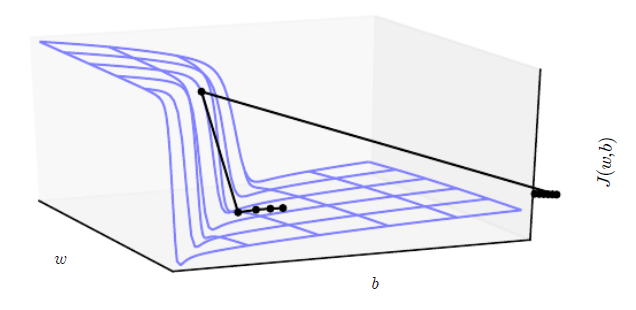
\includegraphics[width=8cm]{figure/cliff2.png}
    \caption{\enquote{The objective function for highly nonlinear deep neural networks or for
recurrent neural networks often contains sharp nonlinearities in parameter space resulting
from the multiplication of several parameters. These nonlinearities give rise to very
high derivatives in some places. When the parameters get close to such a cliff region, a
gradient descent update can catapult the parameters very far, possibly losing most of the
optimization work that had been done} (Goodfellow et al. (2016)).}
  \end{figure}
\end{vbframe}

%%%%%%%%%%%%%%%%%%%%%%%%%%%%%%%%%%%%%%%%%%%%%%%%%%%%%%%%%%%%%%%%%%
%%%%%%%%%%%%%%%%%%          REFERENCES          %%%%%%%%%%%%%%%%%%
%%%%%%%%%%%%%%%%%%%%%%%%%%%%%%%%%%%%%%%%%%%%%%%%%%%%%%%%%%%%%%%%%%
\begin{vbframe}
\frametitle{References}
\footnotesize{
\begin{thebibliography}{99}
%%%%%%%%%%%%%%%%%%%%%%%%%%%%%%%%%%
\bibitem[Ian Goodfellow et al., 2016]{1} Ian Goodfellow, Yoshua Bengio and Aaron Courville (2016)
\newblock Deep Learning
\newblock \emph{\url{http://www.deeplearningbook.org/}}
%%%%%%%%%%%%%%%%%%%%%%%%%%%%%%%%%%
\bibitem[Yann Dauphin et al., 2014]{2} Yann Dauphin, Razvan Pascanu, {\c{C}}aglar G{\"{u}}l{\c{c}}ehre, Kyunghyun Cho, Surya Ganguli, Yoshua Bengio (2014)
\newblock Identifying and attacking the saddle point problem in high-dimensional non-convex optimization
\newblock \emph{\url{https://arxiv.org/abs/1406.2572}}
%%%%%%%%%%%%%%%%%%%%%%%%%%%%%%%%%%
\bibitem[Hao Li et al., 2017]{2} Hao Li, Zheng Xu, Gavin Taylor, Christoph Studer, Tom Goldstein (2017)
\newblock Visualizing the Loss Landscape of Neural Nets
\newblock \emph{\url{https://arxiv.org/abs/1712.09913}}
%%%%%%%%%%%%%%%%%%%%%%%%%%%%%%%%%%
\bibitem[Koenigsberger, 1997]{2} Konrad Koenigsberger (1997)
\newblock Analysis 2, Springer
%%%%%%%%%%%%%%%%%%%%%%%%%%%%%%%%%
\bibitem[Ge (2016)]{1} Rong Ge (2016)
\newblock Escaping from Saddle Points
\newblock \emph{\url{http://www.offconvex.org/2016/03/22/saddlepoints/}}

\end{thebibliography}
}
\end{vbframe}

\endlecture
\end{document}
